%all examples and code taken from High Integrity Software - The SPARK Approach to Safety and Security by John Barnes

\section{Tools}
\label{sec:tools}
In diesem Abschnitt werden die Teile von SPARK behandelt, die sich auf den Korrektheitsbeweis beschäftigen und die damit verbundenen Tools vorgestellt.

Für beweise gibt es folgende Annotationen
\textcolor{red}{einfügen}

\textcolor{red}{Kapitelübersicht siehe S 216}

\subsection{Motivation}
\begin{figure}[h]
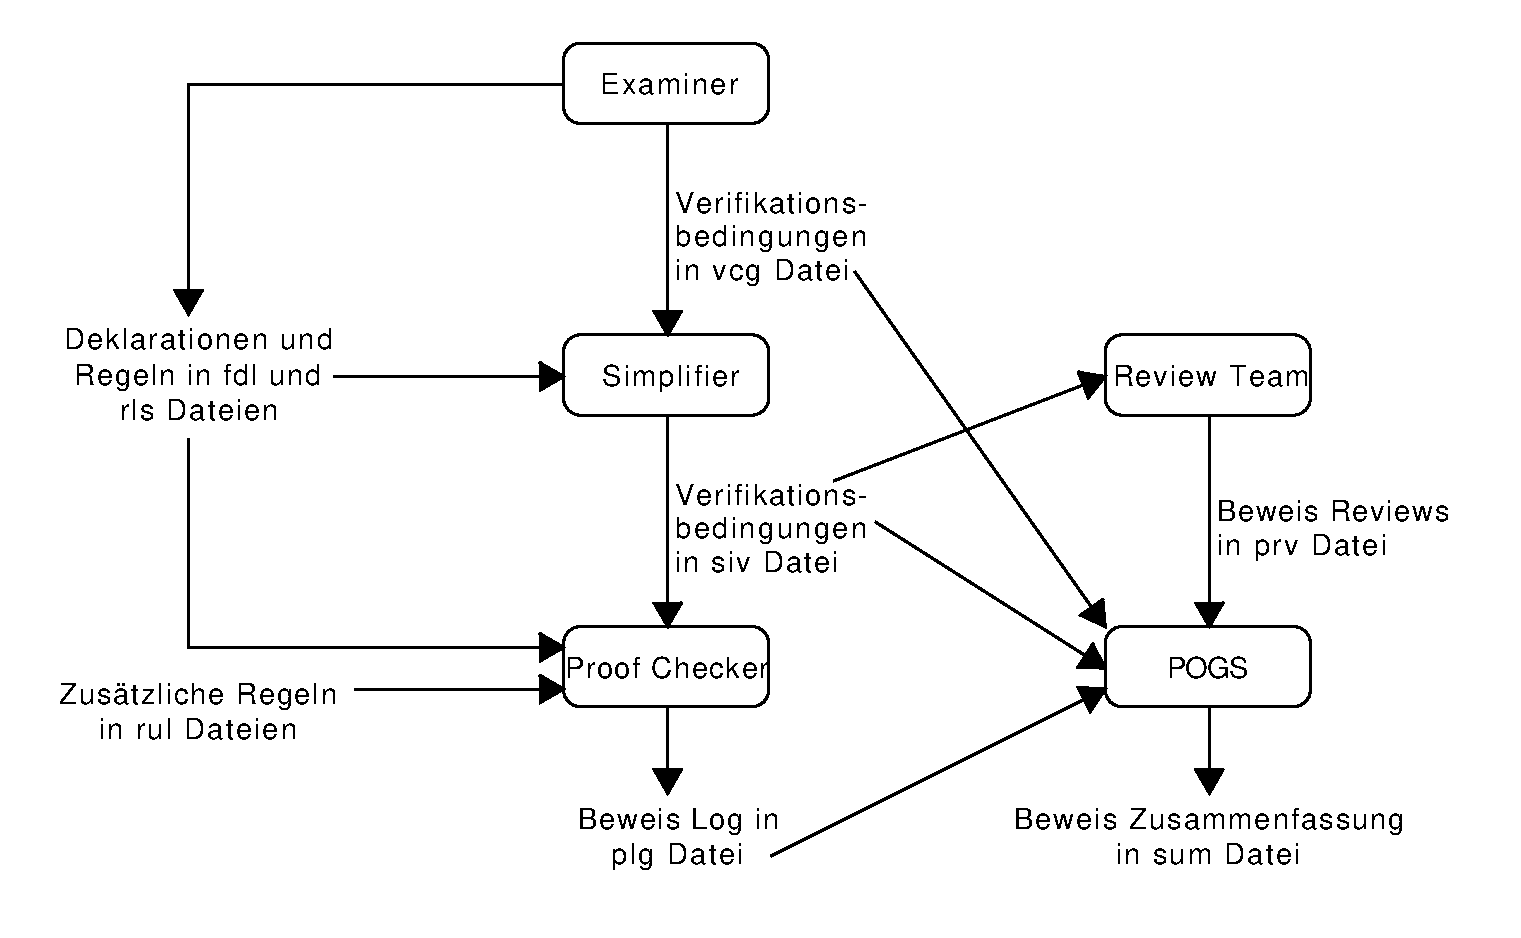
\includegraphics[width=\textwidth{}]{images/ProofProcess.pdf}
\label{fig:proofProcess}
\caption{Der gesamte Beweisprozess}
\end{figure}
Theorie hinter beweisverfahren der quelle entnehmen

\subsection{Examiner}
\label{sec:examiner}
Das wichtigste Tool ist der SPARK Examiner, der es erlaubt Programme abhängig von ihrer Wichtigkeit auf drei Ebenen zu analysieren. Die niedrigste Stufe ist dabei die \textbf{Datenflussanalyse}. Hier wird überprüft, dass Parameter und globale Variablen korrekt genutzt, Variablen nicht vor einer Wertzuweisung gelesen werden, Werte nicht ungenutzt bleiben, usw. Die derives Annotation wird bei der Flow Analyse ignoeriert.
Diese spielen erst bei der \textbf{Informationsflussanalyse} eine Rolle, welche die Norm für die meißten Programme darstellt. Es wird eine Datenflussanalyse durchgeführt und weiterhin wird die derives Annotation ausgewertet. Dadurch wird erkannt, wenn Variablen und Parameter korrekt genutzt werden. Da nur die statischen semantischen Beziehungen betrachtet werden und nicht dynamische Werte, wird diese Analyse auch manchmal flache Verfifikation genannt.
Bei sehr kritischer Software kommen Verifikationskonditionen, Flussanalyse und Beweis Annotationen zum Einsatz.

\subsubsection{Ausführungsreihenfolge}
Der Examiner überprüft ob Quelltexte, die mehrere Kompilierungseinheiten enthalten können, den Regeln von SPARK folgen. Dazu muss es, ähnlich wie beim Compiler, möglich sein auf andere Einheiten, die referenziert wurden, zuzugreifen. Dabei gibt es folgende Regeln:

\begin{itemize}
\item Um den Package Body zu analysieren braucht der Examiner Zugriff auf die Package Spezifikation und die Spezifikation privater Kinder.
\item Um eine Paket Spezifikation oder ein main Unterprogramm, dass von anderen Paketen erbt, zu analysieren braucht der Examiner Zugriff auf die Spezifikationen der anderen Pakete und deren Überklassen.
\item Zur Analyse einer Kind Einheit (child unit) wird die Elternspezifikation benötigt.
\item Für Subunits ist der Zugriff auf die einschließende Unit nötig. 
\end{itemize}
Der Examiner wird über die Komandozeile mit den zu analysierenden Dateien aufgerufen. Er analysiert die Einzeldateien in der gegebenen Reihenfolge. Dabei ist darauf zu achten, dass die Reihenfolge richtig gewählt ist und Abhängigkeiten entsprechend aufgelöst werden können. Für jede Quelldatei wird ein Listing File mit Fehler- und Warnmeldungen und einem Report der Analyse angelegt.
Mit folgendem Aufruf kann solch eine Analyse gestartet werden:
\begin{verbatim}
spark stack.ads stack.adb gobtween.ads gobtween.adb main.ada
\end{verbatim}
Es werden ein Report \texttt{spark.rep} und die drei Listing Dateien \texttt{main.lst},  
\texttt{stack.lst}, \texttt{gobtween.lst} erstellt.
Aufgrund der Abhängigkeiten müssen (im Gegensatz zur Kompilierung) bei einer Änderung alle Dateien neu vom Examiner betrachtet werden.

\subsubsection{Nachrichten}
Die Analyse des Examiner läuft in mehreren Schritten ab. Zunächst wird eine lexikographische und Syntaxanalyse durchgeführt. Dabei werden auchdie Abhängigkeiten aufgelöst. Die Ausgabe in Form von Fehler- und Warnmeldungen ähnelt der eines Compilers. In dieser Phase werden auch Inkonsistenzen in Bezug aud Annotationen aufgedeckt.
Interessanter wird es bei der Flussanalyse. Die Analyse wird in Unterprogrammblöcken ausgeführt.
Die Ausgaben haben folgende Form:
\begin{verbatim}
+++		Flow analysis of subprogramm Push performed: no errors found.
\end{verbatim}

Wurde das Package \texttt{The\_Stack} initialisiert kommt die folgende Meldung:

\begin{verbatim}
+++		Flow analysis of package initialization performed: no errors found.
\end{verbatim}

Einige Beispiele für Fehlernachrichten:
\begin{verbatim}
!!! (1)	Flow Error : 10 : Assignment to A is ineffective.
!!! (2) Flow Error : 33 : The variable A is neither referenced nor exported.
\end{verbatim}

\subsubsection{Optionen}
Wir beschränken uns an dieser Stelle auf eine tabellarische Übersicht der wichtigsten Optionen.
\textcolor{red}{Tabelle!!!}

\begin{footnotesize}
\begin{tabular}{|p{30mm}|p{30mm}|p{30mm}|p{30mm}|}
\hline 
Option & Abkürzung & Default & Beschreibung \\ 
\hline 
Analyse Optionen: \newline syntax\_check \newline flow\_analysis \newline vcs \newline rtc \newline exp\_checks & /sy \newline /fl=type \newline /vc \newline /rt \newline /e & information & nur Syntax check \newline Information oder Datenflussanalyse; Typ kann data oder information sein \newline produziert Verifikationsbedingungen \newline vcs und runtime Checks \newline rtc und overflow Checks \\ 
\hline 
nigger & nigger & nigger & nigger \\ 
\hline 
\end{tabular} 
\end{footnotesize}

\subsubsection{Metadateien und Indexdateien}
Ab einer gewissen Projektgröße wird es zu umständlich alle Dateinamen für den Examiner anzugeben. Hier schaffen Meta- und Indexdateiene Abhilfe.

Eine \textbf{Metadatei} ist eine simple Textdatei, die pro Zeile den Namen einer Quelldatei enthält. Ein Beispiel ist die Datei \texttt{meta.smf}

\begin{verbatim}
--metafile
stack.ads
stack.adb
gobtween.ads
gobtween.adb
main.ada
\end{verbatim}

Der Aufruf wird damit verkürzt auf:

\begin{verbatim}
spark @main.smf
\end{verbatim}

Es ist möglich eine Hierarchie von Metadateien zu erzeugen. Sind andere Metadateien enthalten, so müssen diese das Prefix @ haben. Das vorherige Beispiel könnte mit einer \texttt{stack.smf} und einer \texttt{gobtween.smf} umstrukturiert werden zu

\begin{verbatim}
--nested metafile
@stack.smf
@gobtween.smf
main.ada
\end{verbatim}

Mit dem Zusatz \texttt{\/l=} kann explizit der Name für die Listing Ausgabe angegeben werden.

Eine \textbf{Indexdatei} assoziiert Kompilierungseinheiten mit den Dateien, die sie enthalten. Für das bekannte Beispiel könnte diese Datei folgenden Inhalt haben:

\begin{verbatim}
The_Stack	specification	is in	stack.ads
The_Stack	body			is in	stack.adb
Go_Between	specification	is in	gobtween.ads
Go_Between	body			is in	gobtween.adb
Main		main_program	is in	main.ada
\end{verbatim}

Das main Programm kann dann mit dem Kommando
\begin{verbatim}
spark /index_file=example.idx main.ada
\end{verbatim}
analysiert werden. Bei diesem Aufruf wird nur das Listing für \texttt{main} erstellt und alle Informationen über Fehler in den Abhängigkeiten sind im Report zu finden.

Die Syntaxregeln für eine Indexdatei sind:
\textcolor{red}{Punkte weg und pipe striche richtig!!!!!!!!!!!!!!!!!!!!}
\begin{itemize}
\item index\_file ::= [super\_index] {index\_entry}
\item super\_index ::= superindex is in file\_spec
\item index\_entry ::= file\_entry | component\_entry
\item file\_entry ::= unit\_name entry\_type is in file\_spec
\item entry\_type ::= auxindex | main\_program | specification | body | subunit
\item unit\_name ::= Ada\_unit\_name
\item component\_entry ::= unit\_name components are unit\_name {, unit\_name}
\end{itemize}

Ein Superindex wird durchsucht, wenn die Suche in regulären Indexdateien fehlschlägt. Damit können Indexe hierarchisch strukturiert werden. Gibt es mehrere Dateien, die in mehreren Projekten immer wieder benötigt werden, so können diese beispielsweise in einer Datei \texttt{library.idx} abgelegt werden.

\begin{verbatim}
Spark_IO specification is in sparkio.ads
Spark_IO body is in sparkio.adb
Spark_Elementary_Functions specification is in sparkef.ads
...
\end{verbatim}

Der index eines Projekts kann dann anfangen mit:

\begin{verbatim}
superindex is in library.idx
...
\end{verbatim}

Da es möglich ist Dateien in subunits zu unterteilen, können diese natürlich auch in Indexdateien angegeben werden.

\begin{verbatim}
...
The_Stack body is in stacksep.adb
The_Stack.Push subunit is in push.adb
The_Stack.Pop subunit is in pop.adb
...
\end{verbatim}

Ein alternativer Ansatz ist es eine extra Indexdatei für \texttt{The\_Stack} anzulegen (z.B. \texttt{stackaux.idx}).

\begin{verbatim}
The_Stack body is in stacksep.adb
The_Stack.Push subunit is in push.adb
The_Stack.Pop subunit is in pop.adb
\end{verbatim}

Die Hauptdatei sieht dann entsprechend so aus:

\begin{verbatim}
The_Stack specification is in stack.ads
The_Stack auxindex is in stackaux.idx
...
\end{verbatim}

\texttt{Push} kann dann mit dem Aufruf

\begin{verbatim}
spark /i=main.idxpush.adb
\end{verbatim}

analysiert werden.
Der Examiner stellt zunächst fest, dass er den body von \texttt{The\_Stack} benötigt. Dieser kann im Index nicht gefunden werden und daraufhin wird der Auxiliary file durchsucht.

Es wäre weiterhin möglich \texttt{main.idx} zum Superindex zu machen und die anderen Angaben in \texttt{stackadb.idx} zu machen. Generell gibt es scheinbar keine Konventionen für das Anlegen der Indexdateien und man sollte sich nach der Struktur des jeweiligen Projektes richten. Schleifenabhängigkeiten sind zu vermeiden, da diese nicht vor dem Aufruf entdeckt werden und somit zu einer Dauerschleife führen.

\subsubsection{Beispiel Report}
Das hier gezeigte Report Beispiel zeigt die genutzen Optionen und Dateien und fasst alle Fehler und Warnungen zusammen. In der Spezifikation von Spark\_IO gibt es zwei Warnungen. Die erste bezieht sich auf die with clause für Ada.Text\_IO. Die Warnung kommt zustande, da die Spezifikation dem Examiner nicht zur Verfügung stand.
Die zweite Warnung zeigt, dass die privaten Teile von Spark\_IO versteckt sind.

Es ist möglich Warnungen zu unterdrücken indem eine Kontrolldatei für die Warnungen mitgegeben wird. Diese hat die Endung \texttt{.wrn} und enthält die Typen der zu unterdrückenden Warnungen.

\begin{verbatim}
**********************************************************************
Report of SPARK Examination
SPARK95 Examiner with VC and RTC Generator Release 6.3 / 11.02
Demonstration Version
**********************************************************************

DATE : 16-NOV-2002 13:45:12.26

Options:
index_file=DIALOG.IDX
nowarning_file
notarget_compiler_data
noconfig_file
source_extension=ADA
listing_extension=LST
nodictionary
report_file=SPARK.REP
no_html
nostatistics
fdl_identifiers
flow_analysis=information
ada95
annotation_character=#
profile=sequential

Selected files:
DIALOG.ADA

Index Filename(s) used were:
C:\PRAXIS\DIALOG.IDX
C:\PRAXIS\INVENT.IDX
C:\PRAXIS\COMMON.IDX

No Meta Files used

Full warning reporting selected

Source Filename(s) used were:
C:\PRAXIS\DIALOG.ADA
C:\PRAXIS\INVENT.ADS
C:\PRAXIS\SPARKIO.ADS

Source Filename: C:\PRAXIS\INVENT.ADS
No Listing File

Unit name: Inventory
Unit type: package specification
Unit has been analysed, any errors are listed below.

1 error(s) or warning(s)
Line
37 end Inventory;
^1
--- ( 1) Warning:394:Variables of Type
Inventories cannot be initialized using the
facilities of this package.

Source Filename: C:\PRAXIS\SPARKIO.ADS
No Listing File

Unit name: Spark_IO
Unit type: package specification
Unit has been analysed, any errors are listed below.

2 error(s) or warning(s)

Line
24 with Ada.Text_IO;
^1
--- ( 1) Warning : 1 : The identifier Ada is
either undeclared or not visible at this point.

308 end Spark_IO;

--- ( 2) Warning : 10: The private part of
package Spark_IO is hidden - hidden text is 
ignored by the SPARK examiner.

Source Filename: C:\PRAXIS\DIALOG.ADA
Listing Filename: C:\PRAXIS\DIALOG.LST

Unit name: Dialogue
Unit type: main program
Unit has been analysed, any errors are listed below.

2 error(s) or warning(s)

Line
52 while True loop
^1
!!! ( 1) Flow Error : 40 : Exit condition is stable, of
index 0.

72 end Dialogue;

--- ( 2) Warning : 400: Variable Found is declared
but not used.

--End of file-------------------------------------------
\end{verbatim}

\subsubsection{Beweis Optionen}
Der Examiner erstellt neben den Listings und Reports auch Dateien mit Pfadfunktionen und Verifizierungsbedingungen.

Die Optionen \texttt{/vc}, \texttt{/rtc} und \texttt{/exp} erzeugen Verifikationsbedingungen auf verschiedenen Ebenen. Die Option \texttt{/vc} erzeugt die üblichen Bedingungen und weitere für run-time Checks. Dabei wird eine Datei mit der Endung \texttt{.vcg} erstellt.
Es werden weitere Dateien erstellt, wie in Abbildung ~\ref{fig:examinerFiles} gezeigt wird.

\begin{figure}[h!]
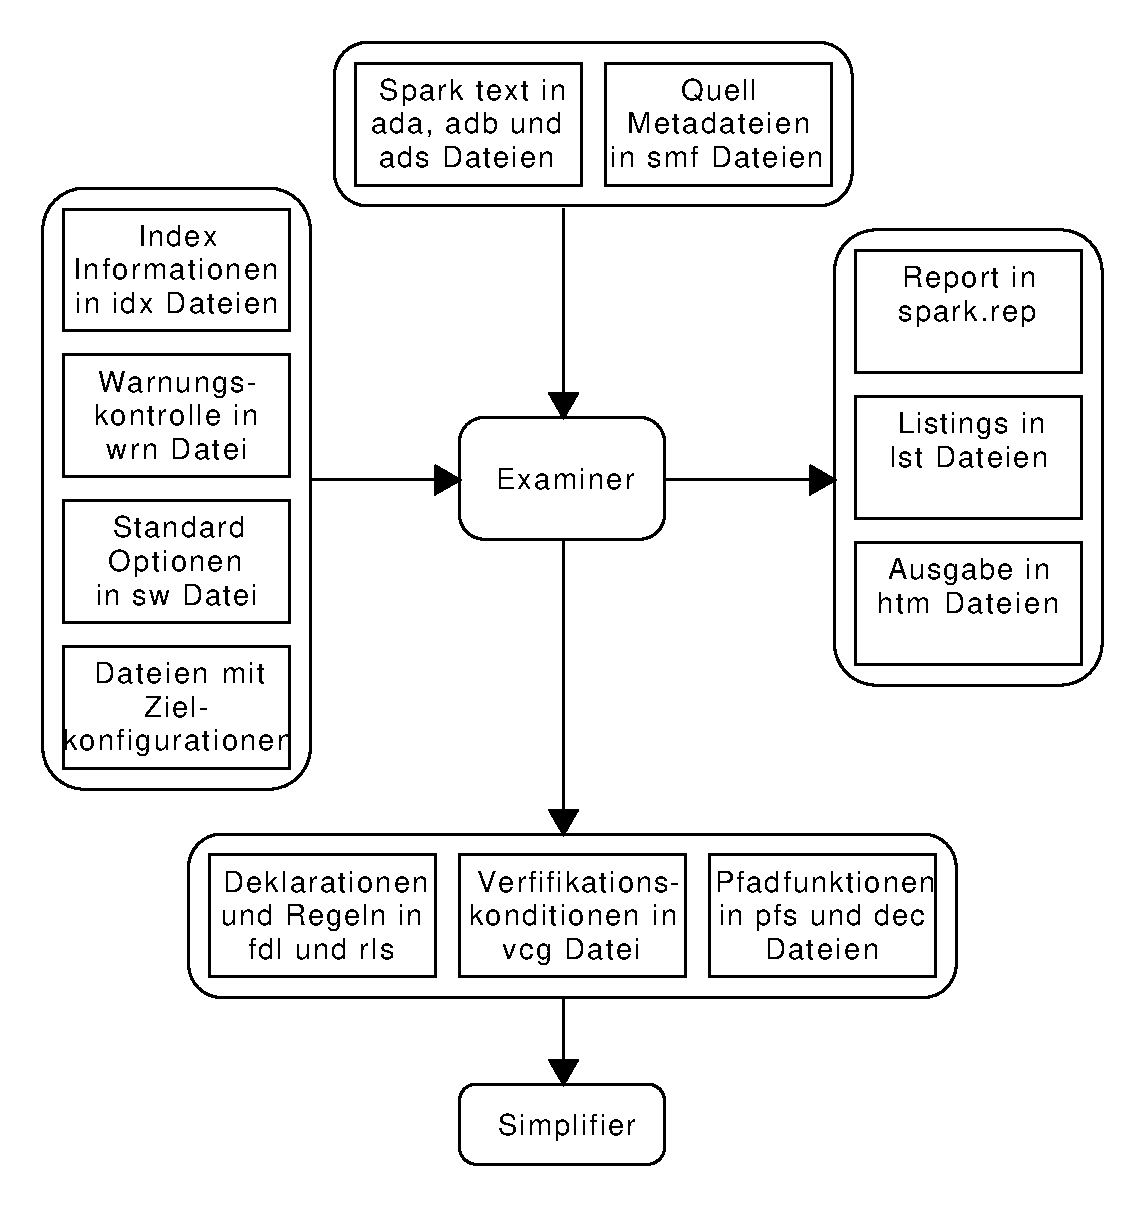
\includegraphics[width=\textwidth{}]{images/examinerFiles.pdf}
\label{fig:examinerFiles}
\caption{Der Examiner mit den zugehörigen Dateien.}
\end{figure}

\subsection{Simplifier}
Der Examiner erzeugt für jedes analysierte Unterprogramm eine \texttt{vcg} Datei mit rohen Verifikationsbedingungen. Diese sind in einer Baumstruktur angeordnet. Weiterhin werden \texttt{fdl} und \texttt{rls} Dateien erstellt, die Informationen zu den Objekttypen und deren Regeln zur Manipulation enthalten. Diese Dateien bilden den Input für den \textbf{Simplifier}.
Der Aufruf des Simplifiers erfolgt ebenfalls in der Konsole und ist einfacher zu Handhaben als der Examiner, da es weitaus weniger Konfigurationsbefehle gibt. Für eine Datei \texttt{example.vcg} mit den entsprechenden \texttt{fdl} und \texttt{rls} Dateien im selben Ordner ist der Aufruf

\begin{verbatim}
spadesimp example
\end{verbatim}

Die vereinfachten Verifikationsbedingungen werden in einer \texttt{siv} Datei gespeichert. Ein Log wird in einer \texttt{slg} Datei angelegt.
Mit dem Aufruf
\begin{verbatim}
sparksimp
\end{verbatim}
werden im aktuellen Verzeichnis und allen Unterverzeichnissen automatisch alle Dateien bearbeitet.

Der Simplifier kann auch Pfadfunktionen vereinfachen, dazu muss beim Aufruf einer \texttt{pfs} Datei die Dateiendungmit angegeben werden. 

\subsection{Proof Checker}
Die Arbeit des Proof Checkers verläuft nicht komplett automatisch, da dies den Rahmen des möglichen sprengen würde. Das Tool ist sehr komplex und mächtig, deswegen können hier nur die Grundzüge erläutert werden.

Ein wichtiger Aspekt des Proof Checkers ist das Logging. Im Log enthalten sind die Hypothesen und Regeln, die füreinen Beweis genutzt wurden und eine Übersicht über die noch zu erledigenden Beweise.
Der Proof Checker wendet einen Satz von Regeln und Strategien an um seine Arbeit zu verrichten. Exemplarisch seien hier einige Regeln genannt. Es gibt simple arithmetisiche Regeln.
\begin{verbatim}
arith(3): X + 0 may_be_replaced_by X.
assoc(4): A*(B*C) may_be_replaced_by (A*B)*C.
distrib(1): A*(B+C) & A*B + A*C are_interchangeable.
\end{verbatim} 
Weiterhin können Regeln auch Bedingungen haben, wie im folgenden Beispiel:
\begin{verbatim}
arith(12): (X/Y)*Y may_be_replaced_by X if [Y<>0].
\end{verbatim}
Es können auch Fakten aus anderen Fakten abgeleitet werden:
\begin{verbatim}
odd(5): odd(X) may_be_deduced_from [odd(-X)].
\end{verbatim}

In der gleichen Datei können beliebig viele Regeln jeder Art gespeichert werden.
Bei der deklaration eigener Regeln ist undbedingt auf deren Korrektheit zu achten, da sonst das ganze Konzept des Proof Checkers ad absurdum geführt würde.

\subsection{Proof Obligation Summarizer}
Nachdem der Simplifier seine Arbeit verrichtet hat, kann der Proof Obligation Summarizer(\textbf{POGS}) mit
\begin{verbatim}
pogs
\end{verbatim}
aufgerufen werden. Das aktuelle Verzeichnis wird dann nach relevanten Dateien durchsucht. POGS erstellt daraus eine Zusammenfassung in einer \texttt{sum} Datei. Diese enthält eine komplette Analyse der Situation. Gezeigt werden die Verifikationsbedingungen, die eliminiert bzw. bewiesen wurden, wie sie bewiesen wurden und was noch bewiesen werden muss.